\scanpage{36}
\margin{\unsure{permuter|puis --} $\longleftrightarrow$}

2) Soit $\Gamma=\mathbb D_n$ \uline{($n\geq3$)}, \deleted{Alors} $\inserted{\Gamma^+\simeq\mathbb Z/n\mathbb Z}$ le ss-gpe car. d'indice 2,
$T=\inserted{Z(\Gamma^+)}$ l'unique tore maximal qui

\[
\begin{aligned}
Z(\Gamma)&=\deleted{\unsure{\mathbb D}}\deleted{\unsure{\{1\}}}\,{}_2T\simeq\{\pm1\}\\ 
\inserted{\mathrm{Aut}(G,\Gamma)=}N(\Gamma)&=\begin{cases}\Gamma&\text{si }n\text{ pair}\\ \Gamma\cdot{}_2T&\text{si }n\text{ impair}\end{cases}\\ 
N(\Gamma)/Z(\Gamma)&\ \deleted{\unsure{\simeq N}}\deleted{\unsure{=\mathrm{Aut}(\Gamma)|\simeq\mathrm{Aut}(\Gamma)}}\ \inserted{\unsure{\simeq}}\ \Gamma/{}_2\Gamma^+\overset{\deleted{\unsure{\sim}}}{\subset}\mathrm{Aut}(\Gamma)
\end{aligned}
\]

\margin{\uline{vérifier}}

\figure{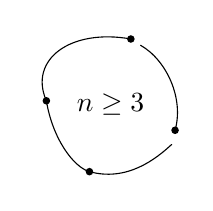
\begin{tikzpicture}[scale=.72,line cap=round]
\draw (.36,1.21) .. controls (-.7,1.4) and (-1.45,.85) .. (-1.13,.12) .. controls (-1.02,-.55) and (-.65,-1.05) .. (-.37,-1.13) .. controls (.29,-1.31) and (.80,-.91) .. (1.08,-.65);
\draw (.53,1.10) .. controls (.99,.84) and (1.30,.16) .. (1.14,-.40);
\foreach \x/\y in {.36/1.21,-1.13/.12,-.37/-1.13,1.14/-.40}{\fill (\x,\y) circle(1.9pt);}
\node at (0,.05) {$n\geq3$};
\end{tikzpicture}}

\uline{Corollaire} \inserted{Sur $S$ sch de car. 0, si $n$ pair} La cat. des $(G,\Gamma)$, $G$ forme de
$\mathrm{GP}(1)$, $\Gamma\subset G$ \deleted{ss-gpe fini ét.} \inserted{forme de $\mathbb D_n$} ($n$ fixé $\geq\unsure{4|3}$)
équivaut à celle des rev. principaux de
$S$ de gpe $\mathbb D_n$, \deleted{\unsure{ou}} ou à celle des \uline{polygones}
réguliers sur $\underline S$ de degré $n$.

% slanted
\margin{\deleted{\unsure{c'est toujours la pp. de le munir de l'un des $\Delta$…}} Il faut \unsure{sans|sans la} donnée d'une solution de l'équation \unsure{$n$-ième cyclotomique|la cyclotomique} pour ``polygône régulier'' pair,}

\inserted{Ou encore, si une racine primitive $n$-ième de 1 est fixée sur $S$,}
Si $n$ est impair $\geq3$, il faut faire des prod
de la cat. des rev. $\Gamma$ princip. \unsure{avec} par celle des
rev. quadratiques, i.e. on
trouve la $\simeq$ description
que pour \deleted{\unsure{du}} $\Gamma=\mathbb D_{2n}$.

% slanted
\margin{\unsure{lorsqu'on sera plus facile|lorsqu'on sera plutôt parti} d'un système de sommets satisfaisant certaines conditions…}

4 \& 5) Soit $\Gamma\simeq\mathcal A_4$ ou $\unsure{\mathfrak S_4|\mathscr S_4}$

\[
\begin{aligned}
Z(\Gamma)&=1\\ 
\inserted{\mathrm{Aut}(G,\Gamma)=}N(\Gamma)&=N\simeq\mathfrak S_4\\ 
N(\Gamma)/Z(\Gamma)&\simeq N(\Gamma)\xrightarrow{\sim}\mathrm{Aut}(\Gamma)
\end{aligned}
\]

\uline{\unsure{Corres.|Coros.|Cor.}} 1:1 entre \deleted{ss-gpes} formes de $\mathbb D_2$, de $\mathcal A_4$,
de $\mathfrak S_4$, contenues dans $G$ fixé
(forment un $\simeq$ espace homogène sous $G$)

\uline{Cor} Equiv. entre catégories, sur base $S$ de
car. 0, des $(G\supset\Gamma)$, $G$ forme de $\mathrm{GP}(1)$, $\Gamma$
forme de $\mathbb D_2$, ou $\mathcal A_4$, ou $\mathfrak S_4$, et avec la
cat. des torseurs sous $\mathfrak S_{4S}$, ou celle
des rev. étales de degré 4, ou celle des
tétraèdres au dessus de $\underline S$, ou celle des
octaèdres au dessus de $\underline S$, ou des formes
de $\mathcal A_4$, ou de $\mathfrak S_4$, sur $\underline S$.

% archive sheet number: 35
